\documentclass[a4paper]{article}
\usepackage{ctex}
\usepackage{multicol}
\usepackage{fancyhdr}
\usepackage{color}
\usepackage{CJK}
\usepackage{amsmath}
\usepackage{graphicx}
\usepackage{algorithm}%写算法时需要调用的包
\usepackage{algorithmic}%写算法时需要调用的包
\usepackage{setspace}%修改行间距需要调用的包
\usepackage{graphicx}
\usepackage{listings}

\definecolor{gray}{RGB}{192,192,192}%灰色设置
\title{\heiti \Large 我的五子棋AI果然有问题}%题目
\author{\songti \small 韩梓辰\ 夏星晨\ 周贤玮\ 赵云龙\ 张坤龙}%作者信息
\pagestyle{fancy}
\lhead{\textcolor{gray} {Computer Science 计算机科学}}
\rhead{\textcolor{gray} {\thepage}}
\renewcommand{\headrulewidth}{0.4pt}
\begin{document}
\maketitle %标题
\thispagestyle{fancy} %页眉
\lhead{\textcolor{gray} {计算机科学}}
\rhead{\textcolor{gray} {DOI:xxxxxx}}
\renewcommand{\headrulewidth}{0.4pt}
\begin{abstract}
    近年来,AlphaGo在棋坛上打遍天下无敌手,甚至进军电子竞技行业,人工智能在发展到今天,人类在竞技体育领域可能越来越不是他们的对手。但是,显然光对胜利的渴求并不新颖,因为人工智能现在越来越多的在各个领域聪明,从以前的人工智障变成了人工智能,在去年,日本一个公司开发了一款人工智能,号称史上最弱人工智能,这个人工智能在几百万次的游戏对战中只获取了1000次的胜利,无论人类如何放水,这个人工智能反倒越来越弱。于是放弃原有的老套人工智能思路,改为设计“人工智障”成为了一个全新的设计思路。\par
该五子棋“人工智障”将基于Python编程语言,通过数学建模,博弈树,神经网络等算法实现。使用pytorch工具,CUDA加速实现矩阵运算的优化,更加优秀的卷积神经网络设计等方法对其进行进一步的优化。最后,在通过大量的人机对战、机机对战、预设对战的数据的学习下,该人工智障已具备一定的计算机科学技术上的智能水平,具有了一定的研究与使用意义。
    \par\textbf{关键词:\ }人工智能,五子棋,神经网络,人工智障,TensorFlow
\end{abstract}
\setlength{\baselineskip}{20pt}
\tableofcontents  %表示目录部分开始
\newpage
    \begin{multicols}{2}
    \section{引言}
    在计算机科学高速发展的当代,人工智能的上限已经变成了一个未知数。人工智能之父图灵在1950年曾说过:下棋是很抽象的活动,是机器可以和人竞争的纯智能领域之一。\cite{ref1}自此之后,越来越多的学者开始研发超越人类的AI,攻克那些曾让人类引以为傲的脑力项目。在1997年时, IBM研发的Deeper Blue战胜了当年国际象棋世界冠军卡斯帕罗夫, 成为人工智能挑战人类智慧发展的里程碑。\cite{b1}而2016 年 3 月,谷歌研发的人工智能–阿尔法狗与围棋世界冠军、职业九段棋手李世石进行围棋人机大战,以4 比 1 的总比分获胜,震惊了棋坛;2016 年末 2017 年初,该程序在中国棋类网站上以“大师” (Master)为注册账号与中日韩数十位围棋高手进行快棋对决,连续 60 局无一败绩,当人们知晓的时候,无不对人工智能的力量感到佩服;2017 年 5 月,在中国乌镇围棋峰会上,它与排名世界第一的世界围棋冠军柯洁对战,以 3比 0 的总比分获胜,取得了围棋界的王冠。围棋界公认阿尔法围棋的棋力已经超过人类职业围棋顶尖水平。\cite{b3}人工智能在棋类方面令人诧异的表现将它推上了一个新的高度。时至今日,棋类AI的算法技术趋向成熟,大量的优化算法,学习模型的构建被提出、完善,包括决策树,算杀,A*搜索等等。这让人工智能在棋类方面几乎变得无懈可击。\cite{b2} \par
就在去年,日本“AVILEN”AI技术公司的首席技术官吉田拓真却反其道而行,研发出了一款“最弱AI”。针对这个模型,他构建了五层神经网络,盘面信息为输入层,输出的是棋盘有利度,通过模仿AlphaGO的构建,以及使用的算法,他成功做出了这个号称“史上最弱”的人工智能。他在推特上发表了这款支持人机对战的黑白棋小程序,最终,这个黑白棋AI在上千名网友的挑战下只输了寥寥数次。这打破了原本“创造胜过人类的人工智能”的固有思维模式。然而,出于时间原因,吉田拓真仅制作了黑白棋的AI程序\cite{ref2},而目前,在其他棋类游戏方面的“人工智障”还是一片空白。\par
基于这个创意,本组决定转换方向,即通过反向思路实现,将人工智能彻底做成另一个新的方向,即“人工智障”。我们计划设计一款可以不断的被人类战胜的机器,无论人类如何放水都可以输掉整个比赛。,本组决定以博弈树,极大极小值搜索,算杀等较为普遍的算法为基础,通过更加优秀的数学建模,神经学习网络,底层优化来实现本组预期制作的五子棋“人工智障”。并将以人与AI,AI与AI之间的棋局胜负为指标,来验证本组五子棋AI的优越性。
    \section{相关工作}
    \subsection{python学习}
    由于大家对python编程语言并不是很熟悉,所以在项目初期,我们五个人都进行了python的学习\cite{ref3},通过python的短暂学习,大家均掌握了大部分的python语法,包括pip的安装库,for的高级用法。通过在网站上的学习过程,我们逐渐的学习并熟练了python的过程,我们利用pygame对本次五子棋的图形界面进行了实现。
    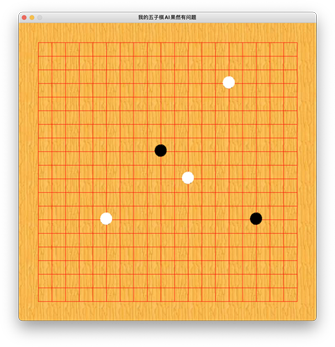
\includegraphics[width=6cm,height=6cm]{gamepic.png}
    此版本游戏实现较为简陋,后期我们对棋子的图片进行了重制,并兼顾了ai的算力的影响等问题,实现了第二版的图形界面,第二版的效果如下:
    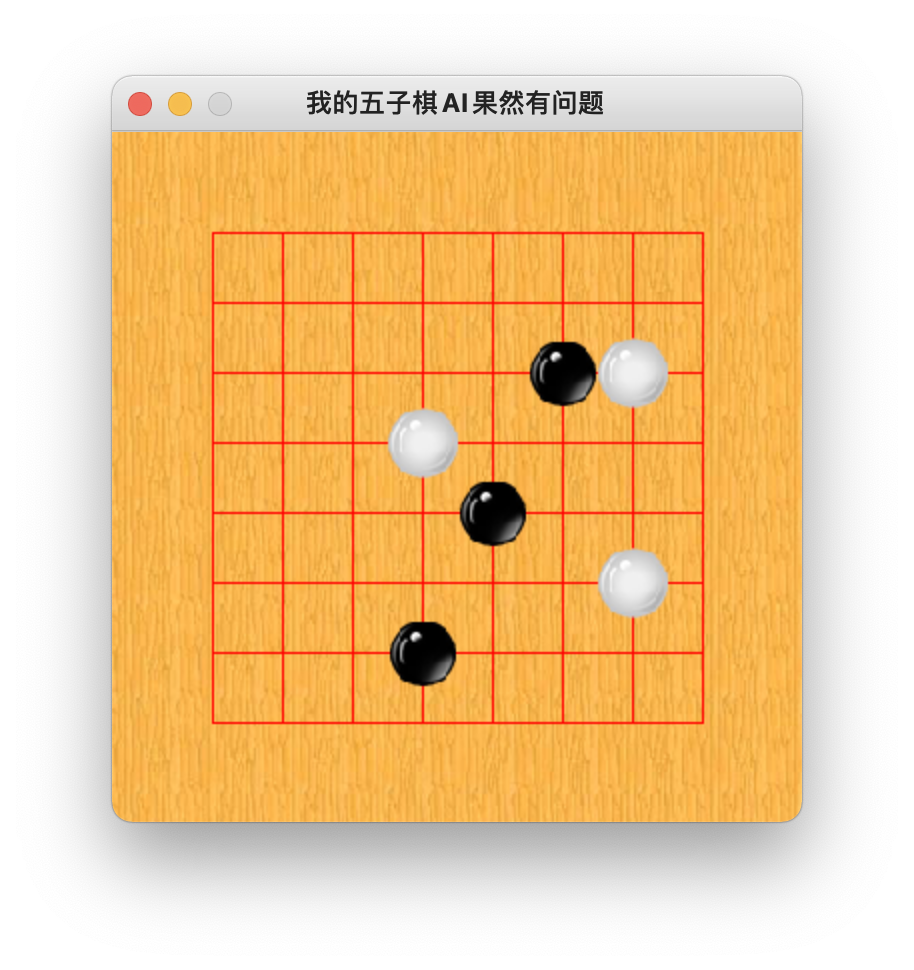
\includegraphics[width=6cm,height=6cm]{game.png}
    \subsection{对照算法}
在训练神经网络之前,我们需要一个标准算法对我们的模型进行训练,这里我们采用的是蒙特卡洛树搜索。
\subsubsection{算法概述}
蒙特卡洛树搜索其实并非什么新型算法,早在上个世纪四十年代,为了满足原子能事业的发展,这个算法就已经被投入使用\cite{k1}。而直到2016 年 3 月,谷歌研发的人工智能–阿尔法狗与围棋世界冠军、职业九段棋手李世石进行围棋人机大战,最终以4 比 1 的总比分获胜,它才引起了人们的注意,网上也开始出现各种博客、论文等详细解析这个算法。时至今日,蒙特卡洛树搜索已经在棋类游戏AI中被广泛使用。\par
蒙特卡洛树搜索实际上是一种随机模拟与树的搜索的结合\cite{k2},它最大的优点它能权衡探索与利用,是一个在搜索空间巨大仍然比较有效的的搜索算法。对于传统的树搜索算法来说,
如果搜索层数较浅,我们就可以照常穷举出所有的情况,得到每一个树节点输赢的概率,然后通过最大最小值搜索得到一个纳什均衡点。然而对于搜索层数比较深的情况(如一
个$10*10$棋盘的五子棋),若要遍历每一个棋局的每一种情况,所有可能的状态将近$3^{100}$个\footnote{对于棋盘上每个点有三种情况:白子,黑子,无子,一共有100个棋格,故大致估算为$3^{100}$种情况(约为$5.15*10^{47}$种情况)},这是现有的计算机无法承受的。这个时候,我们就需要蒙特卡洛树搜索,来帮助我们进行抉择,随机抛弃
一些节点,再进行搜索。这样虽然不能得到所有点的权重,但是可以在有限的时间内换取更多胜率更高的点,从而抛弃大量冗余的节点,节省下大量的时间。
\subsubsection{算法实现}
我们设一个节点i的价值为vi(我们可以使用各种公式来决定函数v,比如最简单的 胜利局数/总局数,或者使用Upper Confidence Bounds(UCB)公式\footnote{Upper Confidence Bounds(UCB)公式:$V_{i}+C*\sqrt{\frac{lnN}{n_{i}}}$)其中 $V_{i}$是节点的估计价值,$n_{i}$是节点被访问的次数,而N则是其父节点已经被访问的总次数。C是一个可调整参数,类似于Perception中的learning rate,它决定了在我们进行蒙特卡洛树搜索时,遍历的次数对该节点估值的影响大小。\par}。大部分的蒙特卡洛树搜索包含一下四个阶段\cite{k3}:\par
1.	选择(Selection)
在这一步,我们会从树的根节点开始,每次都选择一个“最值得我们搜索的点”,即vi最大的子节点,直到我们遇见一个存在未被扩展的子节点的节点。然后我们就对该节点进行扩展。如下图,假设我们遍历到了5号点。\par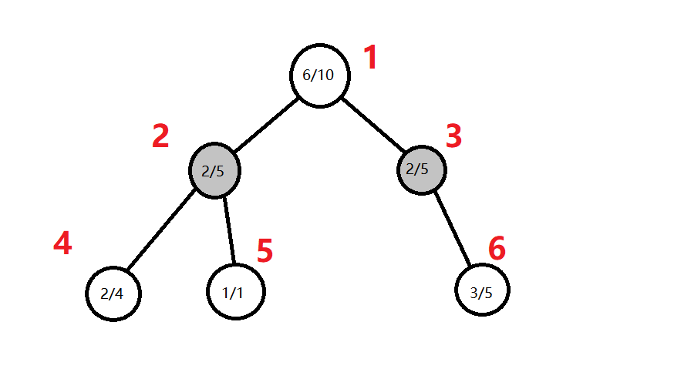
\includegraphics[width=6cm,height=6cm]{k1.png}
2.	扩展(Expansion)
我们新建立一个子节点7作为5号节点的扩展(如图二)。值得注意的是,如果我们当前遍历到的点是白点(这代表此时轮到白方执子),子节点的建立必须是一个黑点(因为此时已经轮到黑方执子)。接着进入第三步模拟。此外,我们的拓展需要有一定的随机性,而非仅仅是按照字典序排序,来保证蒙特卡洛树搜索能充分扩展到“最有搜索价值”的节点\footnote{我们考虑这样一种情况:如果在某一个节点i的胜率很高,可能是50/100,而另一个节点j的胜率也有40/80。那么此时,我们会选择i节点进行扩展。当i节点胜利之后,我们会再次搜索到i节点。如果这次的搜索失败了,那么它的胜率依旧是1/2。在我们不采用随机数的情况下,根据字典序,我们还是会选择节点i来扩展。这就导致了一个循环,i节点在不断被扩展,而j节点一直不会被访问到——即使j的实际胜率可能远远高于i节点。}。\par
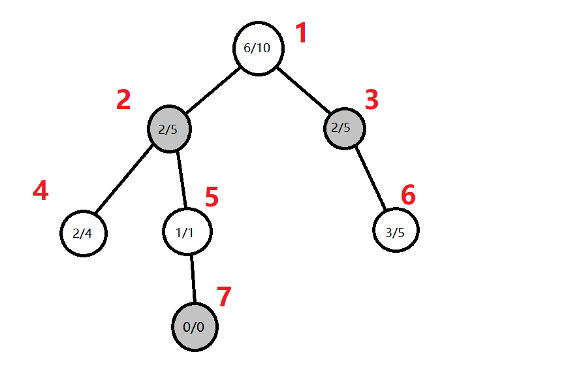
\includegraphics[width=6cm,height=6cm]{k2.png}
3.	模拟(Simulation)
在这个步骤中,我们通过某种特定的下子方法(如仅仅是优秀的随机,甚至于连杀,连防\footnote{连杀、连防:这二者都是五子棋中一种最基础的下法,它不需要大量的思考与计算,但是却非常地接近最优解。所以对于新手而言,连杀与连防是想要下好五子棋必须掌握的策略。具体来说,连杀是指对于进攻方的每一次落子,都能形成活三/眠四/三三/四三/四四,从而逼迫对手进行连防。连防也是一个相似的概念,它是指对于防守方的每一次落子,都能将对手的活二/活三/眠四转变为眠二/眠三/死四。当防守方的防守做得足够优秀,进攻方就无法产生足够大的压力,此时就可以选择一转攻势,通过连杀尝试将对手杀棋。}),来快速走子,获得最后的胜负情况,更新到7节点上(如图3)。\par
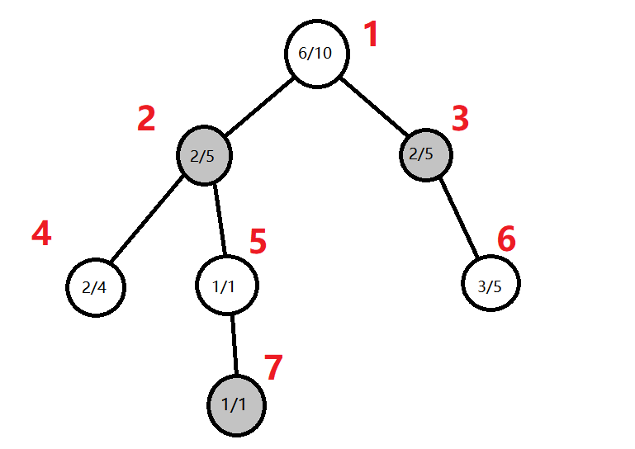
\includegraphics[width=6cm,height=6cm]{k3.png}
4.	反演(Backpropagation)
从7号点出发,将获得的结果回溯到父节点上,更新每一个节点的胜负情况,如图4。需要注意的是,白点代表白子,灰点代表黑子,所以更新的时候若黑点胜利则父白点应记为失败,反之亦然。\par
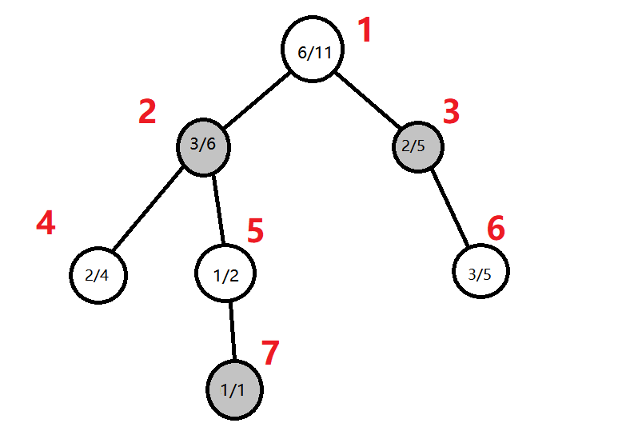
\includegraphics[width=6cm,height=6cm]{k4.png}
5.	重复步骤1。蒙特卡洛树搜索可以在任何时候停止,它的准确度随着搜索时间的增加而收敛。一般来说,我们也会通过设定搜索深度的限制来防止节点任意地拓展,减缓运行的速度。\par
\subsubsection{算法优点}
蒙特卡洛树搜索具有很多的优点\cite{k4}:\par
1.	泛用性。蒙特卡洛树搜索并不要求有太多的专业知识,只要了解了基本的规则,就能很好地完成它的任务。这使得蒙特卡洛树搜索只要稍加更改就能用于另一个模型。\par
2.	非对称的扩展。\cite{k5}MCTS 执行一种非对称的树的适应搜索空间拓扑结构的增长。这个算法会更频繁地访问更加有趣的节点,并聚焦其搜索时间在更加相关的树的部分。非对称的增长这使得 MCTS 更加适合那些有着更大的分支因子的博弈游戏,比如说 19X19 的围棋。这么大的组合空间会给标准的基于深度或者宽度的搜索方法带来问题,所以 MCTS 的适应性说明它(最终)可以找到那些更加优化的行动,并将搜索的工作聚焦在这些部分。
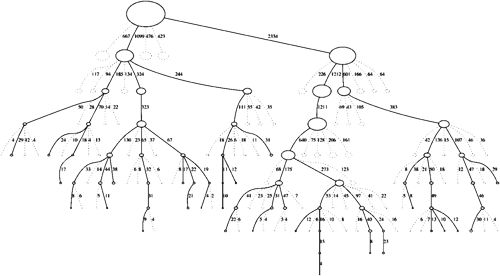
\includegraphics[width=6cm,height=6cm]{k4.jpg}
\par
3.	可被终止。算法可以在任何时候被终止,此时会返回目前所得的最优解。\cite{k6}\par
\subsection{人工智能实现}
基于上述的蒙特卡洛树的算法,我们以此来训练实现我们的人工智能模块。
\subsubsection{实现原理}
对于每一个节点上的状态s,都调用卷积神经网络$f_\theta$进行价值评估和策略评估并使用评估结果作为蒙特卡洛树搜索算法(下称MCTS)的参考。MCTS经过模拟输出状态s下,在不同位置落子的概率$\pi$。其中$\pi$是一个向量,向量值代表MCTS模拟的概率结果。如下所示的向量$\pi_i$,位置(1,3)显示的概率值是0.93,那么表示在该位置落子的可能性非常大。\nextline
$\pi_i$=(0.02,0.03,0.93,…)
\par
经过MCTS模拟得到的策略πi要比仅使用卷积神经网络F评估得到的落子概率P更准确,MCTS通过探索加强了落子概率P的可靠性,这一过程称为策略改善(policy improvement)。以经过MCTS增强的策略巧作为落子依据进行模拟,把模拟最终的结果z作为价值函数的标准.\par
通过采用策略迭代算法去更新卷积神经网络$f_\theta$的参数$\theta$,优化的目标是令卷积神经网络的输出策略概率与价值评估更接近MCTS的模拟结果和博弈最终的胜负结果,即令$f_\theta(s)=(P,v)\rightarrow(\pi,z)$。并且,在每一轮迭代中,总是采用最新的网络参数进行预测和评估。\cite{k7}
本组通过该理论为基础,基于self-play来进行“人工智障”的学习、进化。它不仅是整个训练过程中最耗费时间的步骤,同时也是最关键的步骤。如下是self-play过程的示意图:
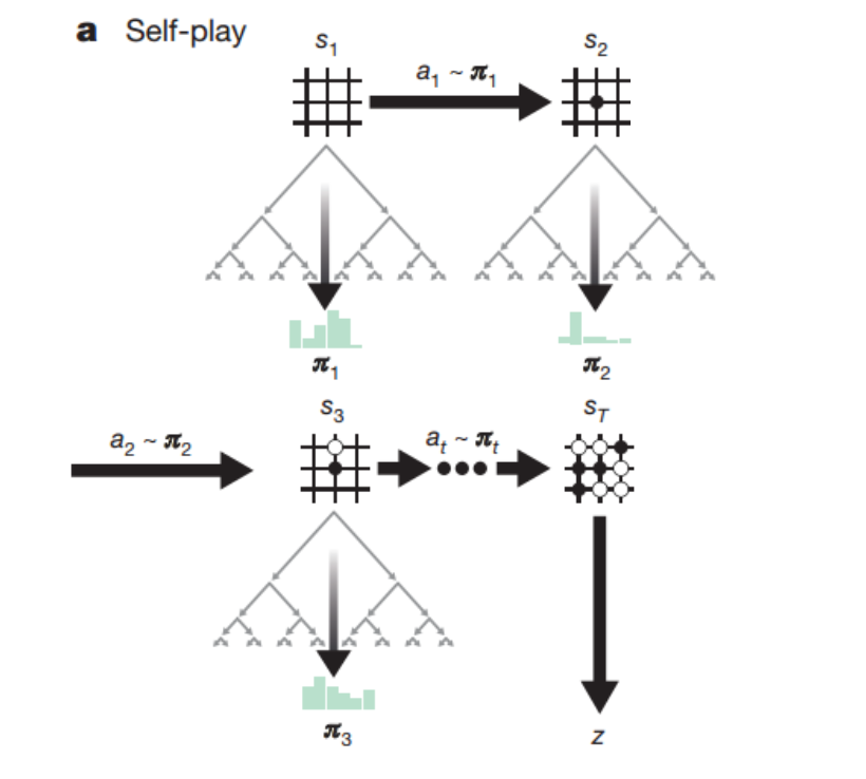
\includegraphics[width=7cm,height=7cm]{AI1.png}
\par
相较于用传统的自我对局,本组通过在自我对局中的以下几个细节处理来实现了对人工智能的优化:\par
1. 通过五子棋本身的性质来扩展训练数据的广度,从而降低训练的重复度。\par
大部分的棋类游戏都具有一定几何上的性质。对于中国象棋来说,它的棋盘在水平翻转和垂直翻转的情况下,局面并不会发生任何的改变。而对于五子棋来说,它的棋盘在经过90°的旋转,以及水平的翻转之后,本质上棋局并不会发生改变。所以我们可以充分利用这一性质来进行我们自我对局的数据库扩展,从而减少不必要的搜索,提高人工智能训练的效率。那么它能够产生多少种相同的局面呢?我们把图像按$0^{\circ}$,$90^{\circ}$,$180^{\circ}$,$270^{\circ}$,以棋盘中心为中心旋转,得到4个图形,每个图形再进行水平翻转,则得到8个图形。当然可能会因为对称或者轴对称,导致其中的一些相同,最终只有4个或者2个甚至1个图形,但是一般情况下我们还是认为这是8个图形。\cite{k8}这样虽然会损失部分的空间利用率,但是却能让代码实现的难度下降一些。从实践角度来说,在每一次的自我对局结束后,我们都会将这一局的棋盘的坐标进行翻转,旋转,从而得到8种相同的棋局,并记录在数据库中,视作人工智能已训练过的棋局。这个优化能够在机器的算力较弱时,以较快的速度获取更多模型的数据,同时也能增加自我对局的数据的准确度与多样化。\par
2.保证数据的统一性来减少每一个节点状态的维数。\par
在自我学习的算法执行过程中,对于每一个局面,我们都会保存大量的数据。我们用$(\pi_i,z_i)$来表示当前局面i的状态,其中πi是根据MCTS的根结点处,对于每一个根节点的访问次数的统计从而计算得到的概率,而zi则是记录下了自我对局的结果。如果我们从两个棋手的视角去表示所得的状态,这实际上和仅仅计算一名棋手的局面是等价的\footnote{五子棋符合博弈树的模型,而博弈树有以下特点,故保存一方的节点与保存双方的节点是等价的:\par
(1)当前的局面就是博弈的初始状态,即作为博弈的初始节点,其它节点是根据规则来扩展出来的局面。\par
(2)博弈树属于一颗与或树,己方掌握着主动权,一直选择最佳的落子点进行扩展,而对方则需要结合这个落子点进行推测落子,也就是说所有的节点的扩展都是以一方的立场进行扩展。\par
(3)博弈树是双方交替落子形成的,叶子节点可以是对方局面,也可以是一方局面,是由模拟的层数决定的。\par
(4)博弈的本原问题是博弈树的扩展是以己方利益最大化来构建的,能使己方获胜和消减对方的着法都需考虑,反之,与此意愿相反的着法都是不可取的\cite{k9}。\par
}。从实现上来说,我们会通过使用两个矩阵来储存两个玩家的位置。假设我们把一个棋手的棋子用第一个矩阵表示,而另一个棋手的棋子用第二个矩阵来表示。在这种情况下,我们会通过i来判断谁是当前的玩家,与此同时,我们的矩阵将会交替表示两个棋手的棋子状态。这对于z来说也是同理,我们可以通过zi=-1,0,1来代表i局面下的棋手失败,和局,以及i局面下的棋手胜利。只不过z必须要通过一个完整的对局结束之后才能被我们确定。\par
3.通过使用最新模型而非最优秀模型从而避免“贪心假象”。\par
在AlphaZero的论文中,通过对比不断维护最优模型进行学习的人工智能与仅仅优化最新模型的人工智能,前者花费了72小时所训练得出的人工智能被后者用仅仅34小时就超越了。\cite{k10} 在AlphaGo Zero模型中,作者通过不断地更新最优秀地模型用于训练当前的人工智能,获得最新的模型,从而希望保证它的准确性。然后每经过一段就通过对比历史模型和最新模型来更新当前最优模型。而到了AlphaZero模型中,我们并不会去更新历史最优模型,作为代替,我们只使用最新的模型作为自我对局的数据获取手段,同时这些数据被用于更新最新的模型。从常理上来说,前者通过不断维护最优秀的模型理应获得更加收敛的结果。而事实上恰恰相反,这种现象被称为“贪心假象”。为了验证这种情况,本组通过对于两种方案的简化与训练,获得了与AlphaZero相似的结果:对于3*3的井字棋的游戏中,如果我们不断更新最优模型,计算机运行了近半个小时才达到井字棋的最优解;而对于只用最新模型生成自我对局的情况下,只需要大约十分钟就能获得最优解。尽管这个测验的数据范围较少,训练时间较短,它依旧可以在一定程度上证明AlphaZero论文中得到的结论。根据本组的猜测,通过新模型产生的数据可能具有更大的多样性,从而导致在这种情况下能遍历到更为广泛的棋局情况。并且当前的最新模型与过去获得的最优模型相差并没有那么大,从而导致自我对局的质量得以保证。同时最新的模型能覆盖到更多特殊的数据,从而加快了人工智能的学习与收敛。\par
4.本组通过对于数据的随机化处理来产生更加具有特殊性的数据,来保证人智能在学习方面不会产生针对某一种局面的部分缺陷。\par
在2017年6月21日,中国棋手王昊洋六段击败了日本围棋程序DeepZenGo,让柯洁惊呼“你是人类的希望”!事实上,在之前的对局中,王昊洋连连败退,直到这一局,他终于引发了DeepZenGo的bug。这是由于这个AI的局部胜率判断错误,导致它在全局采取的策略出现极大的改变,最终败于王昊洋。局后DeepZenGo开发者加藤英树也承认,这是由于该局面的稀有性,导致AI在学习的过程中忽略了这一棋局状态。所以,只有在任何局面下都能正确评估当前局面的优劣以及之后每一步落子的胜率,才能被称作一个优秀的策略价值模型。而对于我们来说,要得到这种策略价值模型,我们应该使用用最新的模型生成的自我对局数据,来帮助人工智能训练到每一个局面。当然,仅仅是这样的优化还不足以遍历到各种各样的局面,所以我们会通过设计一个特殊的拓展策略来扩展到每一种节点,这是不可或缺的。\par
\subsubsection{策略价值网络训练}
我们通过对整个游戏的价值网络训练,以此实现我们的“人工智能”目的:
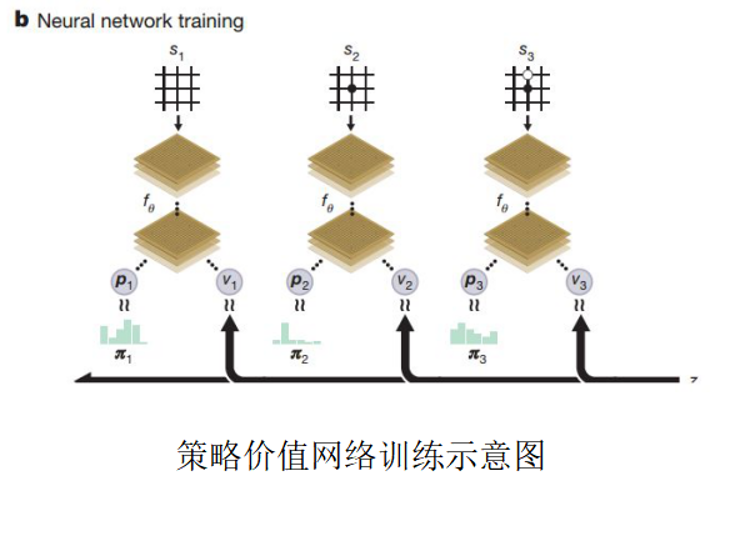
\includegraphics[width=6cm,height=6cm]{AI2.png}
\par
在19路围棋(棋盘由19*19个交叉点组成)中,将每一个交叉点编号,总共可以得到361个编号的交叉点;同时,可以将这361个交叉点映射到361类上,每一个交叉点看做是一类,那么当给定某一特定盘面时,该盘面存在的一种解就是该盘面所属的那一类。这样可以得到运用多分类问题模型给出某一盘面的一个解或多个解的策略网络。策略网络主要解决的是围棋搜索空间太大的问题。每当给定一个特定的盘面,如果不将该盘面所有的落子点作为可能落子点,而是将落子概率最大的几个或十几个落子点作为可能落子点来计算,这样就可以极大的减少搜索空间,提高搜索的效率。\cite{AI1}\par
和围棋类似,五子棋同样可以搭建一个相似的策略价值网络。这个网络可以在读入某一个局面情况时,返回在该局面下每一中落子的胜率以及当前局面的评估。我们就是采用之前自我对局所获得的数据来拓展更新策略价值网络。在这之后,为了获得更加优质的自我对局数据,更新完成的策略价值网络会被我们利用在蒙特卡洛树搜索之后进行的自我对局上。这二者就构成了策略价值网络的螺旋上升,让我们的策略价值网络更加准确和高效。\par
我们将从以下几个方面介绍策略价值网络:\par
1. 用二值特征平面表示某一个局面。\par
AlphaGo Zero一共使用了17个 19*19 的二值特征平面来描述当前局面,其中前16个平面描述了最近8步对应的双方player的棋子位置,最后一个平面描述当前player对应的棋子颜色,也就是先后手。\cite{AI2}而本组在经过一定的考虑之后,简化用于表示棋盘的二值特征平面。本组仅仅将4个二值特征平面投入使用,其中第一个平面表示当前棋手的落子,而第二个平面表示对手的落子,分别使用1/0表示该点有/无子。 根据下五子棋的传统经验,要保证每一步走子尽可能地优秀,一般我们会将子下载敌手上一步执子地附近。所以本组构建了第三个平面,在这个平面上,除了一个位置是1,其他位置均为0,它的意义是敌手最近一步执子的位置。同时,由于在五子棋游戏中,先后手的优势是巨大的,所以我们会采用最后一个平面来表示当前玩家的先后手情况,如果当前执子玩家是先手,则记作1,否则记为0。\par
2. 网络结构的构建。\par
在AlphaGo Zero中,输入局面首先通过了20或40个基于卷积的残差网络模块,然后再分别接上2层或3层网络得到策略和价值输出,整个网络的层数有40多或80多层,更新非常缓慢。\cite{AI2}基于时间消耗的考虑,我们同样简化了该网格结构。我们总共构筑了3层卷积网络,将ReLu作为激活函数,使用32、64、128个filter。同时,我们将输出分为policy和value。在value端,我们会在降维之后链接全连接层,使用非线性函数tanh来给出对于当前局面的评分。而对于policy端,我们同样会在降维之后链接一个全连接层,然后使用softmax函数直接输出每个棋局上每一个节点的落子概率。\par
\subsubsection{训练目标}
	在训练神经网络阶段,使用在蒙特卡洛模拟中生成的数据(S,F,Z)进行训练神经网络模型的参数,目的就是使得对于每个输入的局面S,神经网络的输出策略p和价值v能够和训练样本中的F、Z的差距尽可能地减少,也就是令神经网络的损失函数尽可能地减少。函数如下:\par
$l=(Z-v)^{2}-F^{l}log(p)+c||\theta||^{2}$\par
此损失函数由三部分组成,第一个部分是均方误差损失函数,用于评估神经网络输出的胜负结果与真实对战结果的误差,第二部分采用的是交叉熵损失函数,用于评估神经网络输出的落子策略和MCTS输出的落子策略之间的差异,第三部分则是机器学习中传统的L2正则化项,可以起到防止过拟合的作用。训练的目的就是在自我对战数据集上不断地调整参数,以达到损失函数减少地目的。\cite{k9}\par
通过全面地分析损失函数,我们发现它在一开始剧烈地下降,随后稳定地以一个较低的速率下降,这意味着我们的人工智能所下的子与真实对战越来越接近。同时,我们还会关注策略价值网络输出的落子概率分布的交叉熵的变化情况,在训练开始的一段时间,我们得到的落子概率都是随机的,这导致了交叉熵较大的情况。而随着时间的推移,交叉熵会渐渐变小,这是因为我们的策略网络逐渐学会了在不同的局面下哪些位置能有更大的执子概率。这种落子概率的偏向帮助了蒙特卡洛树搜索过程中能在更加“有趣”的位置进行扩展,得到更高的学习效率。\par
\subsection{人工智障算法思路}
基于人工智能的算法,我们认为人工智障就是对人工智能计算得到的概率矩阵找到其中获胜概率最低的点,然后不断在该点落子即可。\par
我们采用的方法并不是重新搜索最小值,我们采用的是另一个比较简单的思路,我们仍然以棋盘最大值的点为选择,但是我我们在传入概率矩阵的时候




    \section{程序代码}
\begin{lstlisting}
print (hello world)
\end{lstlisting}
    \section{测试}

    \section{结束语}

    \newpage
    \addcontentsline{toc}{section}{参考文献}
    \begin{thebibliography}{30}%参考文献
    \bibitem{ref1}{李金洪\ 深度学习之TensorFlow\ [M]\ .北京.机械工业出版社, 2018-3}
    \bibitem{b1}{ 陈东焰,陆畅.从AlphaGo看机器学习[J].科技创新导报,2020,17(13):146-148. }
    \bibitem{b3}{百度百科 AlphaGo }
    \bibitem{b2}{计算机围棋AlphaGo算法对人类围棋算法的影响[J]. 程思雨,林锋.  中国科技信息. 2019(02)}
    \bibitem{ref2}{naka. J., The weakest Othello, Takujin Yoshida.Thoroughly dig into the inside of the development!(2019-7-25) [2020-09-01]https://ai-trend.jp/business-article/interview/othello-cto-interview}
    \bibitem{ref3}{菜鸟教程 python基础教程 https://www.runoob.com/
    python/python-tutorial.html}
    \bibitem{ref4}{董慧颖;王杨.多种搜索算法的五子棋博弈算法研究[J].沈阳理工大学学报,2017,2}
    \bibitem{k1}{沈大旺.基于人工智能的五子棋搜索算法[J].产业与科技论坛,2020,19(01):73-74.
http://nooverfit.com/wp/%E8%92%99%E7%89%B9%E5%8D%A1%E6%B4%9B%E6%A0%91%E6%90%9C%E7%B4%A2-mcts-%E5%85%A5%E9%97%A8/
}
    \bibitem{k2}{知乎;匿名用户 蒙特卡洛树是什么算法?2017-05-09 https://www.zhihu.com/question/39916945}
    \bibitem{k3}{刘建平Pinard的博客 强化学习(十八) 基于模拟的搜索与蒙特卡罗树搜索(MCTS) 2019-03-04 https://www.cnblogs.com/pinard/p/10470571.html}
    \bibitem{k4}{yif25博客 蒙特卡罗树搜索(MCTS)2018-01-17 16:07 https://www.cnblogs.com/yifdu25/p/8303462.html}
    \bibitem{k5}{知乎; Xiaohu Zhu 蒙特卡洛树搜索简介 https://zhuanlan.zhihu.com/p/30316076}
    \bibitem{k6}{基于蒙特卡洛树搜索的计算机围棋博弈研究[D]. 于永波.大连海事大学 2015}
    \bibitem{k7}{林华. 基于Self-Play的五子棋智能博弈机器人[D].浙江大学,2019.}
    \bibitem{k8}{知乎 叉色-xsir 五子棋的谱库设计与实现 https://zhuanlan.zhihu.com/p/88598278}
    \bibitem{k9}{李昊. 五子棋人机博弈算法优化研究与实现[D].大连海事大学,2020.}
    \bibitem{k10}{David Silver, Aja Huang.Mastering the game of Go with deep neural networks and tree search[J].Nature, 2016, 14(3)}
    \bibitem{AI1}{扶潇. 基于机器学习的围棋策略网络模型的数据优化[D].北京邮电大学,2017.}
    \bibitem{AI2}{CSDN BBlue-Sky AlphaGo Zero详解 https://
    blog.csdn.net/qq\_33813365/article/\par
    details/103344018}





    \end{thebibliography}

    \newpage
\end{multicols}
\end{document}
